\section{Bestimmung der Elementarladung nach Millikan} 

% TODO

\subsection{Vorbereitende Überlegungen}

Zur Vorbereitung dieses Versuches sollte eine Reihe von Aufgaben durchgeführt werden. 
Die Bearbeitung dieser ist im Folgenden dargestellt:
\vspace{0,5cm}

\noindent \textbf{1. Skizzieren sie die Kräftegleichgewichte.}

	Antwort

\noindent \textbf{2. Leiten Sie aus den Kräftegleichgewichten die Formeln für r und Q her.}

	Antwort

\noindent \textbf{3. Schätzen Sie die Dauer der Beschleunigungsphasen nach den Richtungswechseln eines Öltröpfchens mit dem Radius $r = \SI{0,727}{\mu\m}$, indem Sie in beiden Fällen die Gleichung für das Kräftegleichgewicht nach der Geschwindigkeit auflösen und die Beschleunigung abschätzen. Muss die Beschleunigungsphase bei der Zeitmessung berücksichtigt werden?}

	Antwort

\noindent \textbf{4. Warum ist es wichtig, die Kondenstorplatten waagerecht auszurichten?}

	Antwort

\noindent \textbf{5. Warum sind Öltröpfchen besser geeignet als Wassertröpfchen, wenn man bedenkt, dass die Masse der untersuchten Objekte als konstant angesehen wird?}

	Antwort

\noindent \textbf{6. Bewegen sich gering geladene Tröpfchen im elektrischen Feld schneller oder langsamer als stark geladene? Wie ist (qualitativ) dementsprechend die Spannung zu wählen, wenn man gering bzw. stark geladene Öltröpfchen bei etwa gleicher Geschwindigkeit beobachten will?}

	Antwort

\noindent \textbf{7. Welcher Nachteil ergibt sich für die Auswertung, wenn man die fünf Zeitmessungen mit einer Additionsstoppuhr aufsummiert und durch fünf teilt, anstatt alle fünf Werte zu protokollieren und dann zu mitteln?}

	Antwort

\noindent \textbf{8. Wie hängen die Viskosität $\eta$ und die mittlere freie Weglänge $\lambda$ qualitativ von der Temperatur ab?}

	Antwort
	

\subsection{Methoden}

\subsubsection{Aufbau}

\begin{figure}[ht]
	\centering
	\begin{subfigure}{\textwidth}
		\centering
		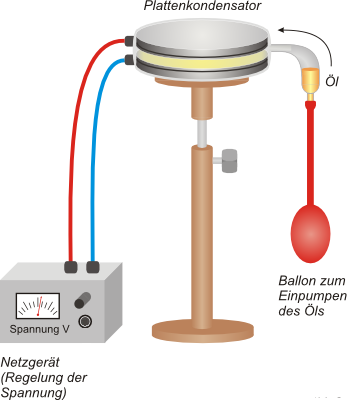
\includegraphics[width=0.5\textwidth]{auswertung/aufbau_1.png}
		\caption{Allgemeine Darstellung des Versuchaufbaus. Zu erkennen ist das Netzgerät mit dem Spannung von bis zu \SI{600}{\volt} für den ebenfalls dargestellten Plattenkondensator, sowie auch die Düse zum Einspritzen des Öls.\cite{Aufbau}}
		\label{fig:aufbau1}	
	\end{subfigure}
	\begin{subfigure}{\textwidth}
		\centering
		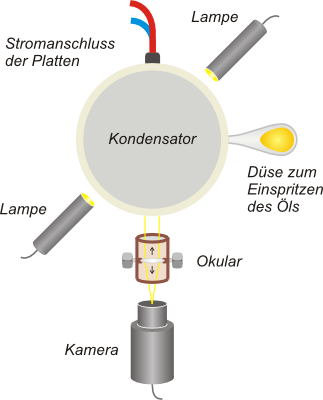
\includegraphics[width=0.45\textwidth]{auswertung/aufbau_2.png}
		\caption{Genauere Darstellung des Aufbaus bezüglich der Betrachtung der Öltröpfchen über das Mikroskop, welches hier aus Kamera und Okular zusammengesetzt ist. Zudem ist die Beleuchtung der Öltröpfchen über die Lampen skizziert.\cite{Aufbau}}
		\label{fig:aufbau2}	
	\end{subfigure}
	\caption{Aufbau des Millikan Versuchs.}
	\label{fig:aufbau}	
\end{figure}

Der Aufbau des Versuches ist in Abb. \ref{fig:aufbau} skizziert. 
Zu erkennen ist der Plattenkondensator, welcher einerseits an ein Netzgerät angeschlossen ist, welches Spannungen von bis zu \SI{600}{\volt} liefern kann, und andererseits an die Düse mit der das Öl in den Plattenkondensator gespritzt wird.
Für die Betrachtung der Öltröpfchen wird ein Mikroskop so an den Plattenkondensator angebracht, dass sich die Tröpfchen in dem Raum zwischen den beiden Platten des Kondensators betrachten lassen. 
Um die Tröpfchen besser zu erkennen wird Licht in den Zwischenraum des Kondensators gestrahlt.

%TODO KOndensator platten Pol gedingse

\subsubsection{Unsicherheiten}

Die bei diesem Versuch auftretenden Unsicherheiten setzen sich aus der Unsicherheit für die Zeitmessung und der des Ortes zusammen.
Für die Zeitmessung dient eine handelsübliche Stoppuhr.
Diese besitzt eine Digitalanzeige und erhält deswegen eine Unsicherheit, welche über eine Rechteckverteilung bestimmt wird.
Da jedoch auch die Reaktionszeit eine Rolle spielt, wird diese mit \SI{0,1}{\second} über eine Dreiecksverteilung bestimmt.
Aus der kombinierten Unsicherheit der Stoppuhr und der Reaktionszeit folgt die der Zeitmessung.
Bei der Unsicherheit des Ortes wird die des Maßes an dem Mikroskop verwendet.
Hierbei handelt es sich um ein Mikrometermaß, welches eine Unsicherheit von \SI{0,1}{\micro\meter} dreiecksverteilt besitzt.
Die Berechnung der kombinierten Unsicherheiten erfolgt nach GUM und ist im Anhang aufgeführt.

\subsection{Durchführung und Datenanalyse}

Damit sich die Elementarladung der Tröpfchen bestimmen lässt, werden zunächst die Geschwindigkeiten $v_{\downarrow}$ und $v_{\uparrow}$ ermittelt.
Dazu wird die Zeit gemessen, welche das Tröpfchen benötigt um zwei Skalenabstände auf dem Mikrometermaß an dem Mikroskop zurückzulegen.
Bei ausgeschaltetem Kondensator, wo die Gewichtskraft $F_\text{G}$ das Tröpfchen nach unten drückt, wird die gemessene Geschwindigkeit $v_{\downarrow}$ genannt.
Umgekehrt $v_{\uparrow}$ für den Fall, dass der Kondensator eingeschaltet ist und die elektrische Kraft $F_\text{E}$ das Tröpfchen nach oben drückt. 
% TODO

\subsection{Diskussion}

% TODO

